50. \begin{figure}[ht!]
\center{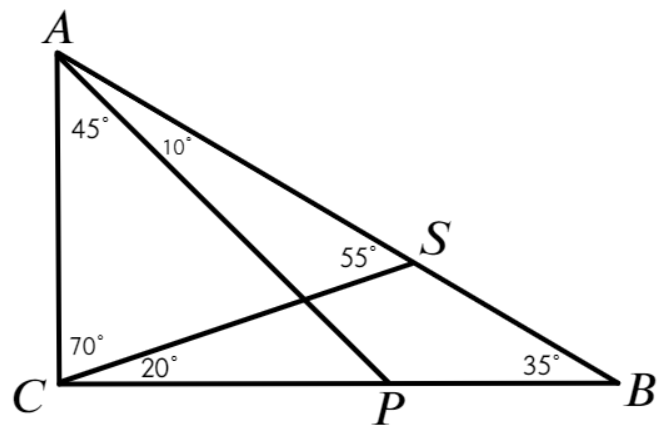
\includegraphics[scale=0.35]{g50.png}}
\end{figure}\\
Посчитаем углы на картинке: $\angle A=90^\circ-35^\circ=55^\circ,\ \angle CAP=55^\circ-10^\circ=45^\circ,\ \angle CPA=90^\circ-45^\circ=45^\circ,\ \angle CSA=20^\circ+35^\circ=55^\circ$ (как внешний в треугольнике $CSB).$ Таким образом, в треугольнике $ACP$ равны углы $CAP$ и $CPA,$ а в треугольнике $ACS$ --- углы $CAS$ и $CSA.$ Значит, эти треугольники являются равнобедренными, ч.т.д.\\
